%%%%%%%%%%%%%%%%%%%%%%%%%%%%%%%%%%%%%%%%%%%%%%%%%%%%%%%%%%%%
% CHAPTER 3 – REQUIREMENT ANALYSIS
%%%%%%%%%%%%%%%%%%%%%%%%%%%%%%%%%%%%%%%%%%%%%%%%%%%%%%%%%%%%

\chapter{Requirement Analysis}

%===========================================================
\section{Introduction to Requirement Analysis}
%===========================================================

This chapter presents a structured and formal specification of the system requirements for the Domavi platform. The purpose of this chapter is to clearly define what the system shall accomplish before proceeding to the system design phase. The requirements documented here serve as a contractual foundation for implementation, validation, and system testing.

The requirement analysis includes requirement elicitation techniques, identification of user classes, use case modelling, functional requirements, non-functional requirements, and external interface requirements. All requirements are written in measurable and testable form using standard requirement engineering principles.

%===========================================================
\section{Requirement Elicitation Techniques}
%===========================================================

This section describes the techniques used to gather and refine the requirements of the Domavi platform. Requirement elicitation ensured that the platform's capabilities are aligned with the real needs of students, young professionals, and landlords.

Requirements for this project were identified using the following techniques:

\begin{itemize}
    \item Informal interviews and discussions with students and young professionals about their experiences finding rooms and roommates.
    \item Analysis of existing solutions such as OLX, Zameen.com, international roommate platforms, and social media housing groups to identify functional gaps.
    \item Literature review of micro-rental and roommate matching systems and their design approaches.
    \item Observation of the current, broker-driven rental workflow to understand pain points around cost, verification, and trust.
    \item Brainstorming and supervisor feedback sessions to refine and prioritise the proposed feature set.
\end{itemize}

%===========================================================
\section{User Classes and Characteristics}
%===========================================================

This section identifies the different categories of users who interact with the Domavi platform. Each user class is defined along with its responsibilities, access privileges, and technical proficiency. This classification supports the role-based access control enforced by the system.

\begin{table}[h]
\centering
\caption{User Classes and Characteristics}

\begin{tabularx}{\textwidth}{|p{3cm}|X|p{2.5cm}|}
\hline
\textbf{User Class} & \textbf{Description} & \textbf{Technical Level} \\
\hline
Tenant & Searches for rooms and roommates, submits booking requests, makes payments, messages landlords, and completes a roommate profile. The primary end user of the platform. & Basic \\
\hline
Landlord & Lists and manages rooms, bed spaces, and hostels, submits ownership and identity documents for verification, and accepts or rejects booking requests. & Basic to Intermediate \\
\hline
Administrator & Reviews and approves verification requests, manages user accounts and status, oversees payments, and monitors platform analytics. & Advanced \\
\hline
External Service & Third-party systems integrated with the platform, including the Google Maps API, cloud media storage, and the email service. & Technical \\
\hline
\end{tabularx}

\end{table}

%===========================================================
\section{System Overview}
%===========================================================

Domavi operates within a layered, client-server architecture designed to support secure, role-based interaction between user interfaces, business logic, and data storage. The React-based presentation layer communicates with a Node.js and Express.js application layer through a RESTful API, and the application layer persists data in a MongoDB database via Mongoose models. The system boundary encompasses all internal modules, namely user and profile management, property listing and search, roommate matching, booking, payment, agreement generation, messaging, and administration, together with the integrated external services for mapping, media storage, and email. Role-based access control governs every protected interaction, ensuring that tenants, landlords, and administrators can only perform actions appropriate to their role.

%===========================================================
\section{Use Case Model}
%===========================================================

The use case model represents the high-level interactions between the actors and the functionalities of the Domavi platform. It defines the system boundary and captures functional behaviour from the perspective of each user.

%===========================================================
\subsection{Use Case Diagram}
%===========================================================

\begin{figure}[h]
\centering
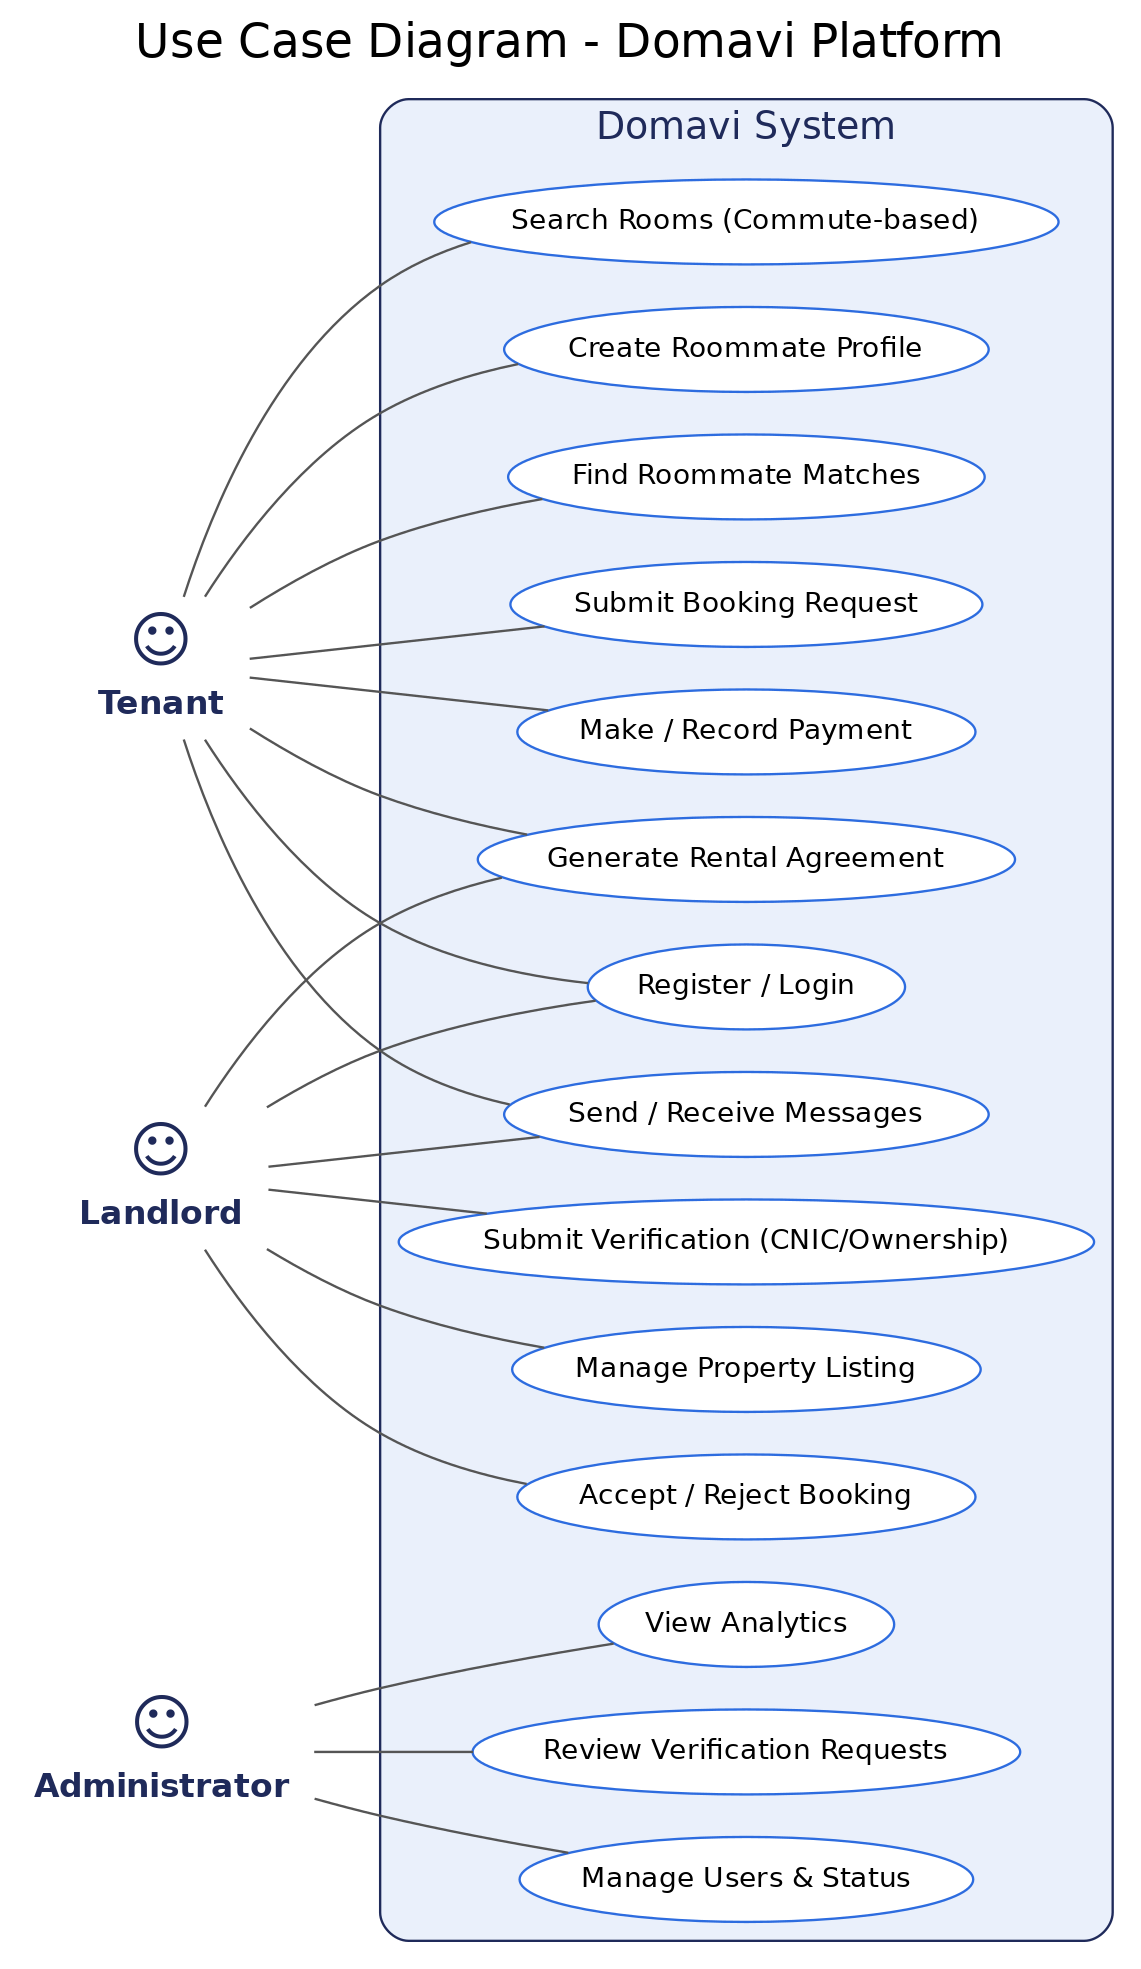
\includegraphics[width=0.6\textwidth]{Figures/usecase_diagram.png}
\caption{Use Case Diagram of the Domavi Platform}
\label{fig:usecase}
\end{figure}

The diagram above illustrates the interaction between the three primary actors, Tenant, Landlord, and Administrator, and the major system functionalities. Common functionality such as registration, login, and verification is shared through \textit{include} relationships, while optional behaviour such as roommate matching extends the core search experience. \textit{(This is a sample diagram from the template; replace it with the finalised Domavi use case diagram before submission.)}

%===========================================================
\subsection{Use Case Descriptions}
%===========================================================

This section provides detailed tabular specifications of the major use cases. These use cases form the basis for deriving the functional requirements presented later in this chapter.

\subsubsection{Module 1: User and Verification}

Below are detailed use cases for registration and verification.

\begin{table}[h]
\centering
\caption{UC-1.1: User Registration}

\begin{tabularx}{\textwidth}{
|>{\raggedright\arraybackslash}p{3.5cm}
|>{\raggedright\arraybackslash}X|}

\hline
\textbf{Use Case ID} & UC-1.1 \\ \hline
\textbf{Use Case Name} & User Registration \\ \hline
\textbf{Actors} & Tenant, Landlord \\ \hline
\textbf{Description} & A new user creates an account and selects a role (tenant or landlord). \\ \hline
\textbf{Trigger} & User selects the ``Sign Up'' option. \\ \hline
\textbf{Preconditions} & User is not already registered with the provided email. \\ \hline
\textbf{Postconditions} & A new account is created with status \textit{pending} and a verification email is sent. \\ \hline
\textbf{Normal Flow} &
\begin{enumerate}
    \item User enters name, email, password, and role.
    \item System validates the input fields.
    \item System creates the account and stores the hashed password.
    \item System sends an email verification link.
    \item Confirmation message is displayed.
\end{enumerate}
\\ \hline
\textbf{Alternative Flow} &
If the email already exists or validation fails, the system displays an appropriate error message.
\\ \hline

\end{tabularx}

\end{table}

\begin{table}[h]
\centering
\caption{UC-1.2: CNIC and Ownership Verification}

\begin{tabularx}{\textwidth}{
|>{\raggedright\arraybackslash}p{3.5cm}
|>{\raggedright\arraybackslash}X|}

\hline
\textbf{Use Case ID} & UC-1.2 \\ \hline
\textbf{Use Case Name} & CNIC and Ownership Verification \\ \hline
\textbf{Actors} & Landlord, Administrator \\ \hline
\textbf{Description} & A landlord submits identity and ownership documents, which an administrator reviews and approves or rejects. \\ \hline
\textbf{Trigger} & Landlord uploads CNIC and ownership proof. \\ \hline
\textbf{Preconditions} & Landlord is registered and logged in. \\ \hline
\textbf{Postconditions} & The verification request is approved or rejected and the user/property status is updated accordingly. \\ \hline
\textbf{Normal Flow} &
\begin{enumerate}
    \item Landlord uploads required documents.
    \item System stores the documents securely and creates a verification request.
    \item Administrator reviews the documents.
    \item Administrator approves or rejects the request.
    \item System updates the verification status and notifies the landlord.
\end{enumerate}
\\ \hline
\textbf{Alternative Flow} &
If the documents are invalid or unclear, the administrator rejects the request with a reason.
\\ \hline

\end{tabularx}

\end{table}

\subsubsection{Module 2: Property and Search}

\begin{table}[h]
\centering
\caption{UC-2.1: Create Property Listing}

\begin{tabularx}{\textwidth}{
|>{\raggedright\arraybackslash}p{3.5cm}
|>{\raggedright\arraybackslash}X|}

\hline
\textbf{Use Case ID} & UC-2.1 \\ \hline
\textbf{Use Case Name} & Create Property Listing \\ \hline
\textbf{Actors} & Landlord \\ \hline
\textbf{Description} & A verified landlord creates a listing for a room, bed space, or hostel. \\ \hline
\textbf{Trigger} & Landlord selects ``Add Property''. \\ \hline
\textbf{Preconditions} & Landlord is logged in and verified. \\ \hline
\textbf{Postconditions} & A new listing is created with status \textit{pending\_verification}. \\ \hline
\textbf{Normal Flow} &
\begin{enumerate}
    \item Landlord enters title, description, type, price, amenities, and location.
    \item Landlord uploads property images.
    \item System validates and geocodes the location.
    \item System saves the listing for review.
\end{enumerate}
\\ \hline
\textbf{Alternative Flow} &
If required fields are missing, the system prompts the landlord to complete them.
\\ \hline

\end{tabularx}

\end{table}

\begin{table}[h]
\centering
\caption{UC-2.2: Commute-Based Property Search}

\begin{tabularx}{\textwidth}{
|>{\raggedright\arraybackslash}p{3.5cm}
|>{\raggedright\arraybackslash}X|}

\hline
\textbf{Use Case ID} & UC-2.2 \\ \hline
\textbf{Use Case Name} & Commute-Based Property Search \\ \hline
\textbf{Actors} & Tenant \\ \hline
\textbf{Description} & A tenant searches for listings near a chosen university or workplace using filters. \\ \hline
\textbf{Trigger} & Tenant enters a location and search criteria. \\ \hline
\textbf{Preconditions} & Active and verified listings exist in the database. \\ \hline
\textbf{Postconditions} & A ranked list of nearby matching listings is displayed. \\ \hline
\textbf{Normal Flow} &
\begin{enumerate}
    \item Tenant enters a target location and filters (price, type, gender preference).
    \item System geocodes the location via the Maps API.
    \item System performs a geospatial query against active listings.
    \item System returns and displays matching listings on a map and list.
\end{enumerate}
\\ \hline
\textbf{Alternative Flow} &
If no listings match, the system displays an empty-state message with suggestions.
\\ \hline

\end{tabularx}

\end{table}

\subsubsection{Module 3: Booking and Roommate Matching}

\begin{table}[h]
\centering
\caption{UC-3.1: Submit Booking Request}

\begin{tabularx}{\textwidth}{
|>{\raggedright\arraybackslash}p{3.5cm}
|>{\raggedright\arraybackslash}X|}

\hline
\textbf{Use Case ID} & UC-3.1 \\ \hline
\textbf{Use Case Name} & Submit Booking Request \\ \hline
\textbf{Actors} & Tenant, Landlord \\ \hline
\textbf{Description} & A tenant requests to book a listing; the landlord accepts or rejects the request. \\ \hline
\textbf{Trigger} & Tenant selects ``Request Booking''. \\ \hline
\textbf{Preconditions} & Tenant is logged in and the listing is active. \\ \hline
\textbf{Postconditions} & A booking record is created with status \textit{pending} and the landlord is notified. \\ \hline
\textbf{Normal Flow} &
\begin{enumerate}
    \item Tenant selects move-in date and submits the request.
    \item System creates a booking with pending status.
    \item Landlord reviews and accepts or rejects the request.
    \item System updates the booking status and notifies the tenant.
\end{enumerate}
\\ \hline
\textbf{Alternative Flow} &
If the landlord rejects the request, the tenant is notified and may search for alternatives.
\\ \hline

\end{tabularx}

\end{table}

\begin{table}[h]
\centering
\caption{UC-3.2: Find Roommate Matches}

\begin{tabularx}{\textwidth}{
|>{\raggedright\arraybackslash}p{3.5cm}
|>{\raggedright\arraybackslash}X|}

\hline
\textbf{Use Case ID} & UC-3.2 \\ \hline
\textbf{Use Case Name} & Find Roommate Matches \\ \hline
\textbf{Actors} & Tenant \\ \hline
\textbf{Description} & A tenant requests a ranked list of compatible roommates based on their lifestyle profile. \\ \hline
\textbf{Trigger} & Tenant opens the ``Roommate Matches'' page. \\ \hline
\textbf{Preconditions} & Tenant has completed a roommate lifestyle profile. \\ \hline
\textbf{Postconditions} & A ranked list of compatible roommate profiles is displayed. \\ \hline
\textbf{Normal Flow} &
\begin{enumerate}
    \item System retrieves the tenant's roommate profile.
    \item System computes weighted compatibility scores against other profiles.
    \item System sorts candidates by score.
    \item System displays the top matches with their compatibility scores.
\end{enumerate}
\\ \hline
\textbf{Alternative Flow} &
If the profile is incomplete, the system prompts the tenant to complete it first.
\\ \hline

\end{tabularx}

\end{table}

%===========================================================
\subsection{Event-Response Table}
%===========================================================

The event-response table defines how the system reacts to significant internal and external events.

\begin{table}[h]
\centering
\caption{Event-Response Table}

\begin{tabularx}{\textwidth}{
|>{\raggedright\arraybackslash}p{3.5cm}
|>{\raggedright\arraybackslash}p{3cm}
|>{\raggedright\arraybackslash}X|}

\hline
\textbf{Event} & \textbf{Source} & \textbf{System Response} \\ \hline

User Login Attempt & Tenant / Landlord / Admin & Validate credentials and grant or deny access based on role. \\ \hline

Document Upload & Landlord & Store CNIC/ownership document securely and create a verification request. \\ \hline

Property Search & Tenant & Geocode the location and return nearby active listings. \\ \hline

Booking Request & Tenant & Create a pending booking and notify the landlord. \\ \hline

Roommate Match Request & Tenant & Compute weighted compatibility scores and return ranked matches. \\ \hline

Payment Submission & Tenant & Record payment details and set status pending until admin confirmation. \\ \hline

\end{tabularx}

\end{table}

%===========================================================
\section{Functional Requirements}
%===========================================================

Functional requirements define the core services and behaviours that the system shall provide. These requirements are derived directly from the use case model presented in Section~3.5. Each requirement is uniquely identified, measurable, and written using formal specification language, and the requirements are categorised by system module.

%===========================================================
\subsection{Module 1: User and Verification Management}
%===========================================================

\subsubsection{FR-1.1 User Registration}

\begin{table}[h]
\centering
\caption{Functional Requirement -- User Registration}

\begin{tabularx}{\textwidth}{|p{3cm}|X|}
\hline
\textbf{Identifier} & FR-1.1 \\
\hline
\textbf{Title} & User Registration \\
\hline
\textbf{Requirement} & The system shall allow users to create an account by providing a name, valid email, password, and role (tenant or landlord). \\
\hline
\textbf{Source} & Stakeholder Requirement \\
\hline
\textbf{Rationale} & Enables authorised, role-based access to platform services. \\
\hline
\textbf{Dependencies} & Database connectivity, email service \\
\hline
\textbf{Priority} & High \\
\hline
\end{tabularx}

\end{table}

\subsubsection{FR-1.2 Multi-Layer Verification}

\begin{table}[h]
\centering
\caption{Functional Requirement -- Multi-Layer Verification}

\begin{tabularx}{\textwidth}{|p{3cm}|X|}
\hline
\textbf{Identifier} & FR-1.2 \\
\hline
\textbf{Title} & Multi-Layer Verification \\
\hline
\textbf{Requirement} & The system shall support email/phone confirmation and allow landlords to submit CNIC and ownership documents for administrator review. \\
\hline
\textbf{Source} & Business Objective BO-3 \\
\hline
\textbf{Rationale} & Establishes trust and reduces fraud on the platform. \\
\hline
\textbf{Dependencies} & Media storage, administration module \\
\hline
\textbf{Priority} & High \\
\hline
\end{tabularx}

\end{table}

%===========================================================
\subsection{Module 2: Property Listing and Search}
%===========================================================

\subsubsection{FR-2.1 Manage Property Listings}

\begin{table}[h]
\centering
\caption{Functional Requirement -- Manage Property Listings}

\begin{tabularx}{\textwidth}{|p{3cm}|X|}
\hline
\textbf{Identifier} & FR-2.1 \\
\hline
\textbf{Title} & Manage Property Listings \\
\hline
\textbf{Requirement} & The system shall allow verified landlords to create, update, and remove listings for rooms, bed spaces, and hostels, including images, price, amenities, and location. \\
\hline
\textbf{Source} & Business Objective BO-1 \\
\hline
\textbf{Rationale} & Provides the supply side of the micro-rental marketplace. \\
\hline
\textbf{Dependencies} & Media storage, Maps API (geocoding) \\
\hline
\textbf{Priority} & High \\
\hline
\end{tabularx}

\end{table}

\subsubsection{FR-2.2 Commute-Based Search}

\begin{table}[h]
\centering
\caption{Functional Requirement -- Commute-Based Search}

\begin{tabularx}{\textwidth}{|p{3cm}|X|}
\hline
\textbf{Identifier} & FR-2.2 \\
\hline
\textbf{Title} & Commute-Based Search \\
\hline
\textbf{Requirement} & The system shall allow tenants to search and filter active, verified listings by proximity to a chosen location, price, room type, and gender preference. \\
\hline
\textbf{Source} & Business Objective BO-4 \\
\hline
\textbf{Rationale} & Enables efficient discovery of relevant accommodation near study or work. \\
\hline
\textbf{Dependencies} & Geospatial index, Maps API \\
\hline
\textbf{Priority} & High \\
\hline
\end{tabularx}

\end{table}

%===========================================================
\subsection{Module 3: Booking, Payment, and Agreements}
%===========================================================

\subsubsection{FR-3.1 Booking Management}

\begin{table}[h]
\centering
\caption{Functional Requirement -- Booking Management}

\begin{tabularx}{\textwidth}{|p{3cm}|X|}
\hline
\textbf{Identifier} & FR-3.1 \\
\hline
\textbf{Title} & Booking Management \\
\hline
\textbf{Requirement} & The system shall allow tenants to submit booking requests and allow landlords to accept or reject them, updating the booking status accordingly. \\
\hline
\textbf{Source} & Business Objective BO-5 \\
\hline
\textbf{Rationale} & Structures and tracks the rental transaction. \\
\hline
\textbf{Dependencies} & Property module, notification service \\
\hline
\textbf{Priority} & High \\
\hline
\end{tabularx}

\end{table}

\subsubsection{FR-3.2 Digital Rental Agreement}

\begin{table}[h]
\centering
\caption{Functional Requirement -- Digital Rental Agreement}

\begin{tabularx}{\textwidth}{|p{3cm}|X|}
\hline
\textbf{Identifier} & FR-3.2 \\
\hline
\textbf{Title} & Digital Rental Agreement \\
\hline
\textbf{Requirement} & The system shall auto-generate a digital rental agreement in PDF format for each confirmed booking, recording the tenant, landlord, property, and terms. \\
\hline
\textbf{Source} & Business Objective BO-5 \\
\hline
\textbf{Rationale} & Automates documentation and provides a verifiable record. \\
\hline
\textbf{Dependencies} & Booking module, PDF generation library \\
\hline
\textbf{Priority} & Medium \\
\hline
\end{tabularx}

\end{table}

%===========================================================
\subsection{Module 4: Roommate Matching}
%===========================================================

\subsubsection{FR-4.1 Roommate Compatibility Matching}

\begin{table}[h]
\centering
\caption{Functional Requirement -- Roommate Compatibility Matching}

\begin{tabularx}{\textwidth}{|p{3cm}|X|}
\hline
\textbf{Identifier} & FR-4.1 \\
\hline
\textbf{Title} & Roommate Compatibility Matching \\
\hline
\textbf{Requirement} & The system shall compute a weighted compatibility score between roommate profiles across lifestyle, preferences, budget, location, and schedule, and return a ranked list of top matches. \\
\hline
\textbf{Source} & Business Objective BO-2 \\
\hline
\textbf{Rationale} & Replaces the roommate ``gamble'' with data-driven matching. \\
\hline
\textbf{Dependencies} & Roommate profile data \\
\hline
\textbf{Priority} & High \\
\hline
\end{tabularx}

\end{table}

%===========================================================
\subsection{Module 5: Communication and Administration}
%===========================================================

\subsubsection{FR-5.1 Secure Messaging}

\begin{table}[h]
\centering
\caption{Functional Requirement -- Secure Messaging}

\begin{tabularx}{\textwidth}{|p{3cm}|X|}
\hline
\textbf{Identifier} & FR-5.1 \\
\hline
\textbf{Title} & Secure Messaging \\
\hline
\textbf{Requirement} & The system shall enable secure, in-app messaging between tenants and landlords and maintain a persistent conversation history. \\
\hline
\textbf{Source} & Stakeholder Requirement \\
\hline
\textbf{Rationale} & Allows coordination without prematurely exposing personal contact details. \\
\hline
\textbf{Dependencies} & Authentication module \\
\hline
\textbf{Priority} & Medium \\
\hline
\end{tabularx}

\end{table}

\subsubsection{FR-5.2 Administration and Analytics}

\begin{table}[h]
\centering
\caption{Functional Requirement -- Administration and Analytics}

\begin{tabularx}{\textwidth}{|p{3cm}|X|}
\hline
\textbf{Identifier} & FR-5.2 \\
\hline
\textbf{Title} & Administration and Analytics \\
\hline
\textbf{Requirement} & The system shall allow administrators to review verification requests, manage user accounts and status, oversee payments, and view platform analytics. \\
\hline
\textbf{Source} & Business Objective BO-6 \\
\hline
\textbf{Rationale} & Provides governance, oversight, and operational insight. \\
\hline
\textbf{Dependencies} & All modules \\
\hline
\textbf{Priority} & High \\
\hline
\end{tabularx}

\end{table}

%===========================================================
\section{Non-Functional Requirements}
%===========================================================

Non-functional requirements define the quality attributes that describe how the system performs. These requirements are measurable and support reliability, usability, performance, security, and maintainability.

%===========================================================
\subsection{Performance Requirements}
%===========================================================

\begin{itemize}
\item PER-1: The system shall load the main dashboard and search results within 3 seconds under normal operating conditions.
\item PER-2: The system shall return roommate match results within an acceptable latency for a typical candidate pool.
\item PER-3: The system shall support multiple concurrent users as defined in the project scope without significant degradation.
\item PER-4: Geospatial search queries shall be optimised through appropriate indexing to ensure responsive results.
\end{itemize}

%===========================================================
\subsection{Security Requirements}
%===========================================================

\begin{itemize}
\item SEC-1: The system shall implement secure authentication using JSON Web Tokens.
\item SEC-2: Passwords shall be stored using a secure hashing algorithm with salting.
\item SEC-3: Sensitive data shall be transmitted over HTTPS.
\item SEC-4: Role-based access control shall be enforced for every protected resource.
\item SEC-5: Verification documents (CNIC, ownership proof) shall be stored securely and accessible only to authorised administrators.
\end{itemize}

%===========================================================
\subsection{Reliability Requirements}
%===========================================================

\begin{itemize}
\item REL-1: The system shall aim to maintain high availability with at least 99\% uptime.
\item REL-2: System failures shall not result in loss of booking, payment, or agreement data.
\item REL-3: Backup and recovery mechanisms shall be in place for the database.
\end{itemize}

%===========================================================
\subsection{Usability Requirements}
%===========================================================

\begin{itemize}
\item USE-1: The interface shall be intuitive and easy to navigate for users with basic digital literacy.
\item USE-2: Clear and meaningful error messages shall be displayed for invalid actions.
\item USE-3: The system shall follow consistent UI/UX design principles across all pages.
\item USE-4: The application shall be fully responsive across desktop and mobile browsers.
\end{itemize}

%===========================================================
\subsection{Scalability Requirements}
%===========================================================

\begin{itemize}
\item SCA-1: The system shall support a growing number of users and listings.
\item SCA-2: The architecture shall allow horizontal or vertical scaling of the application and database.
\item SCA-3: The database design shall support large volumes of listings and roommate profiles.
\end{itemize}

%===========================================================
\subsection{Maintainability Requirements}
%===========================================================

\begin{itemize}
\item MAIN-1: The system shall follow a modular architecture with clear separation of concerns.
\item MAIN-2: Source code shall be written in TypeScript and documented for clarity.
\item MAIN-3: Future features shall be integrable without major restructuring of existing modules.
\end{itemize}

%===========================================================
\section{External Interface Requirements}
%===========================================================

This section defines how the Domavi platform interacts with external entities including users, hardware devices, software systems, and communication networks.

%===========================================================
\subsection{User Interface Requirements}
%===========================================================

\begin{itemize}
\item UI-1: The system shall provide a graphical web interface accessible from modern browsers.
\item UI-2: Standard, readable font sizes shall be used throughout (12--14pt body text).
\item UI-3: The layout shall be responsive across desktop, tablet, and mobile devices.
\item UI-4: Navigation shall remain consistent and role-appropriate across all modules.
\end{itemize}

%===========================================================
\subsection{Hardware Interface Requirements}
%===========================================================

\begin{itemize}
\item HI-1: The system shall operate on standard computing devices with an internet connection.
\item HI-2: The application shall function on devices running modern web browsers without specialised hardware.
\item HI-3: Server hosting shall provide sufficient compute and storage for the database and media.
\end{itemize}

%===========================================================
\subsection{Software Interface Requirements}
%===========================================================

\begin{itemize}
\item SI-1: The system shall interact with a MongoDB database through the Mongoose object data modelling layer.
\item SI-2: The system shall integrate the Google Maps API for geocoding and map display.
\item SI-3: The system shall integrate cloud media storage for images and verification documents.
\item SI-4: The system shall integrate an SMTP email service for verification and notifications.
\end{itemize}

%===========================================================
\subsection{Communication Interface Requirements}
%===========================================================

\begin{itemize}
\item CI-1: The system shall use HTTPS for secure client-server communication.
\item CI-2: RESTful APIs shall be used for all backend communication.
\item CI-3: Real-time messaging shall be supported for in-app conversations.
\item CI-4: All API requests to protected endpoints shall carry a valid authentication token.
\end{itemize}

%===========================================================
\section{Assumptions and Dependencies}
%===========================================================

This section lists the assumptions made during requirement analysis and the external dependencies on which the system relies.

\begin{itemize}
\item The system assumes stable internet connectivity for all online operations.
\item Third-party services (Google Maps API, cloud media storage, email service) are assumed to remain available and within quota.
\item Users are assumed to provide truthful information and possess basic digital literacy.
\item Administrators are assumed to be available to process manual verification requests in a timely manner.
\end{itemize}

%===========================================================
\section{Requirement Traceability Matrix}
%===========================================================

This matrix maps project objectives to use cases and functional requirements to ensure alignment and completeness.

\begin{table}[h]
\centering
\caption{Requirement Traceability Matrix}

\begin{tabularx}{\textwidth}{|p{2cm}|p{3cm}|X|}
\hline
\textbf{Objective} & \textbf{Use Case} & \textbf{Functional Requirement} \\ \hline
BO-1 & UC-2.1 & FR-2.1 \\ \hline
BO-2 & UC-3.2 & FR-4.1 \\ \hline
BO-3 & UC-1.2 & FR-1.2 \\ \hline
BO-4 & UC-2.2 & FR-2.2 \\ \hline
BO-5 & UC-3.1 & FR-3.1, FR-3.2 \\ \hline
BO-6 & UC-1.2 & FR-5.2 \\ \hline
\end{tabularx}

\end{table}

%===========================================================
\section*{Chapter Summary}
%===========================================================

This chapter presented a structured requirement analysis of the Domavi platform.
It defined the requirement elicitation techniques, the user classes (tenant,
landlord, administrator, and external services), and a use case model with
detailed use case specifications for registration, verification, listing,
search, booking, and roommate matching. Functional requirements were specified
module by module, followed by measurable non-functional requirements covering
performance, security, reliability, usability, scalability, and maintainability.
External interface requirements and a traceability matrix linking objectives to
requirements were also included. These requirements form the formal foundation
for the system design presented in the next chapter.
